\documentclass[12pt]{report}			% Začátek dokumentu
\usepackage{MP}							% Import stylu

\author{Alex Olivier Michaud}
\title{Protokoly TCP/IP}
\date{14. února 2023}
\vedouci{ Dr.rer.nat. Mgr. Michal Kočer}
\place{V Českých Budějovicích}
\skolnirok{2022/2023}
\logo{
\includegraphics[scale=1.25]{GJ8_logotyp}}

\begin{document}
\pagenumbering{roman}                   % číslování stránek římskými číslicemi
	\mytitlepage						% Vygenerování titulní strany
	
	\prohlaseni{
		Prohlašuji, že jsem tuto práci vypracoval samostatně s vyznačením všech použitých pramenů.
	}	
	
	\abstrakt{
		Cílem této práce je poskytnout přehled základů komunikace na úrovni TCP/IP. Důraz je kladen na návrh vlastního aplikačního protokolu založeného na rodině protokolů TCP/IP a jeho následnou implementaci. Práce upozorní na klíčové aspekty komunikace v rámci TCP/IP a představí návrh a implementaci nového protokolu pro použití v síťové komunikaci. Ověření funkčnosti protokolu proběhne na jednoduché videohře napsané v Pythonu.				% Abstrakt
	}{
	TCP/IP, Protokol, Sítě, Klient-server, Python, MicroPython						% Klíčová slova
	}
	
	\podekovani{
		Rád bych vyjádřil hlubokou vděčnost Dr.rer.nat. Michalu Kočerovi, vedoucímu mé seminární práce, za jeho odborné vedení, podporu a povzbudivou pomoc po celou dobu mého výzkumu. \\
Chtěl bych také upřímně poděkoval své rodině za její vytrvalou podporu a za korektury mé práce. 						% Poděkování
	}
	
   {\tableofcontents\newpage}			% Obsah
	
\addtocounter{page}{1}		% Posunutí countru stránek
\pagenumbering{arabic}		% Číslování stránke arabskými číslicemi
	\chapter*{Úvod}
	
	Komunikace je základním aspektem moderních technologií a protokol TCP (Transmission Control Protocol) je jedním z klíčových protokolů, které umožňují tuto komunikaci. V této práci se budeme zabývat základy komunikace na úrovni TCP/IP a se zaměřením na jeho praktické využití.
\\
V první části práce uvedeme přehled základů komunikace a úlohy a vlastnosti síťových protokolů při komunikaci.
\\
V další části popíšeme návrh a vývoj vlastního aplikačního protokolu, který je založen na rodině protokolů TCP/IP. Půjde o vývoj jednoduchého aplikačního protokolu, který je určen k usnadnění komunikace mezi mikropočítačem a osobním počítačem.
\\
V hlavní část práce se zaměřemíme na praktickou implementaci navrženého protokolu na konkrétním scénáři síťové komunikace. K tomu použijeme mikropočítač a osobní počítač, aby se demonstrovala funkčnost protokolu v reálném prostředí.
\\
Na závěr provedeme zhodnocení navrženého protokolu, diskusi jeho silných stránek a omezení a navrhneme směry dalšího výzkumu a vývoje.
\\
Cílem této práce je přispět k pochopení protokolu TCP a jeho praktického použití na konkrétním komunikačním scénáři. Práce má být prakticky zaměřená a pomoci studentům získat hlubší znalosti o protokolech TCP.	
	
	
	\part{Základy komunikace aplikací na úrovni TCP/IP}
	
		\chapter{Protokoly TCP/IP}
			
			\section{historie TCP/IP}
				V roce 1966 se povedlo v USA Bobu Taylorovi úspěšně sehnat finance od Charlese Marii Herzfelda, ředitele \texttt{ARPA},\footnote{Nyní známo jako \texttt{DARPA}(Defense Advanced Research Projects Agency) je výkonná moc ministerstva obrany Spojených států amerických, které je pověřena vývojem technologií pro vojenské účely} na projekt ARPANET, který měl umožnit přístup k počítačům na velké vzdálenosti. V dalších třech letech se rohodlo o počátečních standardech pro identifikaci, autentizaci uživatelů, přenos znaků a kontrolu a roku 1969 byl ARPANET poprvé použit firmou \texttt{BBN}. \cite{History}, \cite{History3}, \cite{History2}, \cite{ARPNET} \\
Při dalším výzkumu a pokusech o vytvoření nového modelu ARPANET, dva vědci Robert Elliot Kahn a Vinton Gray Cerf vytvořili nový model, kde hlavní zodpovědnost za spolehlivost byla předána uživateli místo sítě. Tímto roku 1974 vznikl nový protokol Transmission Control Program, který byl vydán v RFC\footnote{žádost o komentáře - označuje dokumenty popisující internetové protokoly} 675 s názvem Specification of Internet Transmission Control Program. Ale tato verze nebyla až do roku 1981 funkční, poté byla zprovozněna verzí 4. Je standardizována pomocí RFC 791 - Internet Protocol(IP) a RFC 793 Transmission Control Protocol(TCP). \cite{History}, \cite{History3}, \cite{History2}, \cite{ARPNET}, \cite{IP}, \cite{TCP}, \cite{Rules}
\\
TCP i IP, prošlo s postupem času velkým vývojem, kdy vznikalo stovky aktualizací. Například roku 1994 vzniklo Internet Protocol next generation (IPng), který zavádí IP verzi 6. Nyní se aktivně používá 10+ variant TCP na Linuxu. MacOS a Windows je má zavedeno jako výchozí nastavení. \cite{History3}, \cite{History2}, \cite{History}, \cite{IP}   

			\section{Základy komunikace aplikací na úrovni TCP/IP }
			TCP/IP je rodina protokolů, která umoňuje komunikaci uzlů\footnote{bod přerozdělení nebo koncový bod komunikace} a to pomocí end-to-end\footnote{snaží se o to, aby důležité role sítě byly řešeny konečným úzlem} principu a specifikováním toho jak by data měla být připravena, adresována, přenášena, směrována a přijmána. Tyto protokoly jsou nejčastěji děleny do čtyř úrovní Link, Internet, Transport a Application. \cite{zakladykomunikace1}, \cite{zakladykomunikace2}, \cite{zakladykomunikace3}
			
			\section{Principy TCP/IP}
			TCP/IP stojí na několika zásadních principech jako klient-server, encapsulace, stateless a robustnost. \cite{Princip5}, \cite{Princip4}
\\
Client-server princip je vztah, kde jeden uzel požádá o službu nebo
 prostředek druhý uzel. V TCP/IP modelu je uživatel klient(je mu poskytována služba) a další počítač je server. \cite{zakladykomunikace1}, \cite{Princip5}, \cite{Princip1}, \cite{Princip3}
\\
Encapsulace je princip, který používá abstraktní dělení TCP/IP do čtyř úrovní. V každé takové úrovni se k původním datům přidávají další data, tak aby mohli být odeslány přes síť. Opačný proces, kdy uživatel se snaží dostat data se nazývá deencapsulace. \cite{zakladykomunikace1}, \cite{Princip5} 
\\
Rodina TCP/IP protokolů je nazývána jako stateless. Tento princip říká, že jakákoliv žádost o službu od uživatele je nezávislá na té předchozí. Toto umožňuje lepší plynulost sítě, jelikož síťové cesty mohou být používány nepřetržitě. \cite{Princip5}
\\
Robustnost je princip, který dbá na to, aby uživatel neposílal žádná data, která by mohla způsobit problém druhému uživateli při procházení TCP vrstvami. Zároveň se snaží předvídat vše co dostane od druhého uživatele, co by mohlo způsobit problém a s případnými problémy nakládá liberálně. \cite{Princip5}, \cite{Princip6}
			
			
			\section{Vrstva síťového rozhraní}
			Vrstva síťového rozhraní je nejnižší úroveň TCP/IP, dělí se na další dvě podkategorie, a to fyzická a logická. \cite{Princip5}, \cite{Link4}
\\
Na fyzické úrovni jsou všechna zařízení, kabely a etc., která konkrétně posílají bity. Protokoly na této úrovni jsou standardizovány \texttt{IEEE}\footnote{Institute of Electrical and Electronics Engineers}, například jsem patří protokol Ethernet\footnote{kabely s kroucenou dvojlinkou}, Wi-Fi, etc. \cite{Princip5}, \cite{Link2}, \cite{Link3}
 \\
Další součastí link úrovně je logická část, tato úroveň protokolů spojuje pouze síťový segment\footnote{část počítačové sítě} a posílá takzvané frame pouze v LAN(lokální síť). Toto propojení zajištuje pomocí různých protokolů, jako například ARP(Address Resolution Protocol), který umožňuje switchy, aby rozpoznal MAC adresy zařízení. Tato část se dále dělí na podčásti a to LLC a MAC podčást. LLC podčást umožňuje adresování a kontrolu logické části. Dále specifikuje mechanismy, pro zařízení, které adresují a kontroluje data, která jsou vyměněna mezi zařízeními. MAC podčást má zodpovědnost za možnost přístupu k mediu (CSMA/CD), nebo tento problém řeší pomocí MAC adres. \cite{Princip5}, \cite{Link2}, \cite{Link3}, \cite{Link4}, \cite{Link5}, \cite{Link6}


			\section{Síťová vrstva}
Síťová vrstva, v referenčním modelu TCP/IP známá také jako vrstva 2, je zodpovědná za směrování a předávání paketů v sítích. Jedná se o důležitý level, který umožňuje zařízením v různých sítích vzájemně komunikovat, díky němuž může fungovat internet. \cite{sit1}, \cite{sit2}
\\
Jedním z hlavních úkolů síťové vrstvy je směrování, které zahrnuje rozhodování o vhodné cestě pro každý paket na základě jeho cíle. K určení nejlepší cesty se používají různé metody a algoritmy pro směrování, od jednoduchých statických metod až po adaptivnější přístupy, které mohou zohlednit různé faktory v síti. \cite{sit1}, \cite{sit2}
\\
Kromě směrování je síťová vrstva zodpovědná také za realizaci předávání paketů v mezilehlých uzlech podél zvolené cesty a také za řízení toku dat a prevenci přetížení sítě. Hraje také klíčovou roli při propojování různých sítí, což umožňuje bezproblémovou komunikaci mezi nimi. \cite{sit1}, \cite{sit2}


			\section{Transportní vrstva}
Transportní vrstva, v referenčním modelu TCP/IP známá také jako vrstva 3, je důležitou součástí procesu síťové komunikace. Je zodpovědná za zajištění spolehlivé komunikace mezi aplikačními procesy běžícími na různých hostitelích v síti. \cite{tran1}, \cite{tran2}
\\
Mezi hlavní úkoly transportní vrstvy patří oprava chyb, segmentace a desegmentace dat a zajištění doručení dat ve správném pořadí. K provádění těchto úkolů používá protokoly, jako je protokol TCP (transmission control protocol) a UDP (user datagram protocol). \cite{tran1}, \cite{tran2}, \cite{tran3}
\\
Transportní vrstva, která se v modelu OSI nachází mezi síťovou vrstvou (vrstva 3) a aplikační vrstvou (vrstva 7), zajišťuje koncové spojení mezi zdrojovým a cílovým hostitelem. To jim umožňuje komunikovat bez rušení jinými síťovými komponenty. \cite{tran1}, \cite{tran2},  \cite{tran3}
\\
Souhrnně řečeno, transportní vrstva shromažďuje segmenty zpráv z aplikační vrstvy a přenáší je do sítě, kde jsou znovu sestaveny a doručeny do aplikační vrstvy cílového hostitele. Je nezbytnou součástí procesu síťové komunikace, poskytuje spolehlivé transportní služby vyšším vrstvám a umožňuje aplikacím komunikovat mezi sebou napříč sítí. \cite{tran1}, \cite{tran2}, \cite{tran3}


			\section{Aplikační  vrstva}
 Aplikační vrstva je v referenčním modulu TCP/IP určena číslem čtyři, ale jelikož je pro mou práci nejdůležitější tak si tuto vrstvu rozdělíme podle podrobnějšího modelu ISO/OSI, kde aplikační vrstva se dělí na vrstvu relační, prezentační a aplikační. 
 
 
				\subsection{Relační vrstva}
Relační vrstva je zodpovědná za navazování, udržování a ukončování komunikačních relací mezi dvěma koncovými body. Zajišťuje, aby komunikace mezi dvěma koncovými body byla spolehlivá a probíhala hladce, i když dojde k chybám nebo přerušení na nižších vrstvách. Například pomocí synchronizace je umožněno do posílaných dat přidat kontrolní body. Díky těmto bodům, v případě chyby, si příjemce může znovu vyžádat poslání dat od určitého bodu. Zároveň umožňuje, aby na stejné přenosové lince probíhalo více komunikačních relací současně, které mohou být duplexní, poloduplexní, či simplexní. \cite{session1}, \cite{session2}


				\subsection{Prezentační vrstva}
Prezentační vrstva je zodpovědná za doručování, formátování a šiforvání informací při jejich předávání mezi různými systémy a aplikacemi. \cite{presentation1}, \cite{presentation2}
\\
Prezentační vrstva zajišťuje, aby syntaxe a sémantika přenášených zpráv byla standardizována a ve správném formátu. Odpovídá za integraci všech různých formátů do standardizované podoby pro efektivní komunikaci a za kódování zpráv z formátu závislého na uživateli do společného formátu a naopak pro komunikaci mezi různými systémy.Pro vytvoření těchto formátu se používají různé serializace, jako například XML či TVL, které umožňují efektivní přenos složitých datových struktur. \cite{presentation1}, \cite{presentation2}, \cite{presentation3}
\\
Kromě serializace je prezentační vrstva zodpovědná také za šifrování a dešifrování dat. To se často provádí za účelem ochrany citlivých informací při jejich přenosu po sítích a může se provádět na různých vrstvách síťového zásobníku v závislosti na konkrétních požadavcích aplikace nebo protokolu. \cite{presentation1}, \cite{presentation2}, \cite{presentation3}


				\subsection{Aplikační vrstva}
Aplikační vrstva se dělí na dva prvky a to CASE\footnote{Common Application Service Element} a SASE\footnote{Specific Application Service Element}. Ty jsou určeny pro lehčí vytváření aplikací, protože poskytují stavební bloky, se kterými aplikace mohou pracovat. CASE poskytuje služby pro aplikační vrstvu a požaduje služby od vrstvy relací. Zatímco SASE poskytuje specifické aplikační služby, jako je přenos souborů, vzdálený přístup k databázi a zpracování transakcí. \cite{aplication1}, \cite{aplication2}, \cite{aplication3}
\\
Dále aplikační vrstva poskytuje několik funkcí, ty umožňují uživatelům snadný přístup k datům a manipulaci s nimi. Dovoluje uživatelům odesílat a přijímat e-maily, přistupovat k souborům na vzdáleném počítači a spravovat je, přihlašovat se jako vzdálený hostitel a přistupovat k informacím o různých službách. Poskytuje také protokoly, které zajišťují softwaru odesílat a přijímat informace a prezentovat uživatelům smysluplná data. \cite{aplication1}, \cite{aplication2}, \cite{aplication3}


			\section{Slovník protokolů a technologií}
			
			
Nyní zde popíšeme několik různých protokolů, ty jsou později konkrétně použité v naší praktické části. Jsou řazeny podle vrstev od nejnižší po nejvyšší a technologie jsou až za nimi.


				\subsection{I2C}
				
				
I2C\footnote{Inter-Integrated Circuit} je protokol používaný pro komunikaci mezi čipy. Tento protokol umožňuje připojit se do sběrnicového rozhraní zabudovaného do zařízení pro sériovou komunikaci. \cite{i2c4}, \cite{i2c1}, \cite{i2c3}
\\
Funguje na prinicipu SDA\footnote{Serial Data} a SCL\footnote{Serial Clock} rozhraní. SDA je využito na komunikaci a přenos dat mezi zařízeními a SCL je užito na přenos hodin. Dále se mezi zařízeními dohodne role Master nebo Slave. Počet obou zařízení Master i Slave je omezen počtem adres. Ale pro naše účely pracujeme s módem pouze jednoho Master zařízení. \cite{i2c4}, \cite{i2c1}, \cite{i2c3}, \cite{i2c4}
\\
 Master zařízení zahájí komunikaci tím, že v kanále SDA změní napětí z vysokého na nízké, a obráceně u kanálu SCL. Nyní Master zařízení pošle Slave zařízením adresu, pokud ta souhlasí, Slave zařízení pošle ACK\footnote{acknowledgement} zprávu. Nyní je komunikace navázána. Dále pokaždé když dostane Master zařízení rámec s daty od Slave zařízení, posílá mu na zpět ACK zprávu. \cite{i2c4}, \cite{i2c3}
\\
Výhody této komunikace jsou v jednoduchosti zapojení, v počtu zařízení v Slave roli a ve spolehlivosti a dostupnosti na mnoha zařízeních.  \cite{i2c1}, \cite{i2c4}


				\subsection{Wi-Fi}
				
				
Wi-Fi je označení zařízení pro přenos dat s danými specifikacemi, která prošla v minulosti testováním jedním ze členů organizace \texttt{Wireless Ethernet Compatibility Alliance} (WECA),  dnes s názvem \texttt{Wi-Fi Alliance}. Tato zařízení využívají standard IEEE 802.11, který umožňuje bezdrátově sdílení dat. Nejpoužívanějšími standardy Wi-Fi jsou 802.11b a 802.11a. \cite{WiFi1}, \cite{WiFi2}
\\
Tyto standardy využívají rádiové vlny k přenosu informací mezi zařízeními a směrovačem prostřednictvím specifických frekvencí. V závislosti na množství přenášených dat lze využít dvě rádiové frekvence: 2,4 GHz a 5 GHz. Standard 802.11b využívá frekvenci 2,4 GHz, zatímco standard 802.11a využívá frekvenci 5 GHz. \cite{WiFi1}
\\
Wi-Fi také využívá různé architektonické postupy, přičemž pro naše účely jsou nejdůležitější přístupové body (AP) a antény\footnote{Ta sice nepoužívá standarty 802.11, nýbrž vzniká kolaborací různých firem, ale pro účely práce má stejné využití, jako wifi}. Metoda AP zahrnuje použití stacionárního přístupového bodu, který funguje jako základní rádiová stanice a datový most, ten je obvykle připojený k síti prostřednictvím technologie Ethernet. Tento přístupový bod také nastavuje potřebná bezpečnostní opatření. \cite{WiFi1}, \cite{Pruvodce}
\\
Technologie antén se často využívá v otevřených venkovních prostorách, kde je nutná komunikace na velké vzdálenosti, navíc se využivají i bleskojistky a přídavné antény. \cite{Pruvodce}


				\subsection{ARP}
				
				
Protokol ARP\footnote{Address Resolution Protocol} je protokol používaný v LAN\footnote{Lokální síť} k určení fyzické adresy zařízení pomocí adresy síťové vrstvy (např. IP adresy). Když chce zařízení komunikovat s jinými ve stejné síti LAN, potřebuje znát cílovou fyzickou adresu, aby mu mohlo poslat data. Má však k dispozici pouze IP adresu cílového zařízení. Zde přichází na řadu protokol ARP. \cite{arp3}, \cite{arp1}
\\
Aby zdrojové zařízení zjistilo fyzickou adresu toho cílového, rozešle všem uzlům v síti LAN paket s požadavkem ARP. Paket obsahuje IP adresu cílového zařízení a žádost o jeho fyzickou adresu. Paket obdrží všechny uzly v síti LAN, ale pouze to se shodnou IP adresou odpoví svou fyzickou adresou. Tato odpověď je odeslána zpět zdroji ve formě paketu odpovědi ARP. \cite{arp3}, \cite{arp2}
\\
Zdrojové zařízení pak uloží fyzickou adresu cílového zařízení do své mezipaměti ARP, což je tabulka, která mapuje IP adresy na fyzické adresy. Tímto způsobem může použít fyzickou adresu z mezipaměti pro budoucí komunikaci s cílovým zařízením, místo aby musel vysílat požadavek ARP pokaždé, když chce odeslat data. Mezipaměť ARP má hodnotu časového limitu, která udává dobu, po kterou zůstane fyzická adresa v mezipaměti, než ji bude třeba obnovit. \cite{arp1}, \cite{arp2}, \cite{arp3}

				\subsection{IP}
				
				
Internetový protokol (IP) je klíčovou součástí internetu, která je zodpovědná za směrování datových paketů mezi zařízeními v síti. \cite{IP2}, \cite{IP3}, \cite{IP4}
\\
Jedním z hlavních úkolů protokolu IP je přenášet datové pakety, nazývané IP datagramy, přes mezilehlé uzly k jejich cíli. K tomu protokol IP využívá informace o topologii sítě, takzvaně směrovací informace, které rozhodují o dalším směru přenosu IP datagramu. Tento proces se nazývá směrování. \cite{IP2}, \cite{IP3}, \cite{IP4}
\\
Protokol IP pracuje s abstraktními adresami, takzvanými adresami IP, což jsou 32bitová čísla, která identifikují zařízení v síti. Tyto adresy se používají k určení cesty, kterou mají datové pakety projít, aby dosáhly svého cíle. Aby bylo možné přenášet data mezi zařízeními v různých sítích, spoléhá protokol IP na překlad síťových adres. Protokol IP slouží k převodu mezi adresami IP a fyzickými adresami, například adresami sítě Ethernet. \cite{IP2}, \cite{IP3}, \cite{IP4}
\\
Protokol IP může pracovat ve spolehlivém nebo nespolehlivém režimu. Ve spolehlivém režimu je protokol IP zodpovědný za správné doručení datových paketů a podnikne kroky k opravě případných chyb. V nespolehlivém režimu protokol IP jednoduše zahodí všechna poškozená data a pokračuje dál, opravu chyb přenechá protokolům vyšších vrstev. Nespolehlivý režim je obecně efektivnější, protože snižuje dobu spojenou s opravou chyb. \cite{IP2}, \cite{IP3}, \cite{IP4}
\\
Kromě směrování datových paketů a adresování poskytuje protokol IP také možnosti fragmentace a opětovného sestavení. To umožňuje protokolu IP přenášet datové pakety, které jsou větší než maximální přenosová jednotka sítě, jejich rozdělením na menší pakety a jejich opětovným sestavením v cíli. \cite{IP1}, \cite{IP2}, \cite{IP3}, \cite{IP4}


				\subsection{TCP}
				
				
Protokol TCP\footnote{Transmission Control Protocol} je základní součástí internetu a zajišťuje spolehlivý přenos dat mezi zařízeními. Je to protokol zaměřený na spojení, což znamená, že navazuje a udržuje spojení mezi zařízeními nebo aplikacemi, dokud nedokončí výměnu dat. \cite{Pruvodce}, \cite{TCP}, \cite{TCP1}
\\
Protokol TCP je zodpovědný za rozdělení původní zprávy do paketů, jejich očíslování a předání vrstvě IP k transportu do cílového zařízení. Dále se stará o přenos případných odložených paketů, spravuje řízení toku a zajišťuje, aby všechny pakety dosáhly svého cíle.  \cite{Pruvodce}, \cite{TCP}, \cite{TCP1}
\\
K navázání spojení mezi zařízením a serverem používá protokol TCP třícestný handshake, který zajišťuje současný přenos více spojení soketů TCP v obou směrech. Zařízení i server musí před zahájením komunikace synchronizovat a potvrdit pakety a poté mohou vyjednávat, oddělovat a přenášet spojení soketů TCP. \cite{Pruvodce}, \cite{TCP}, \cite{TCP1}, \cite{TCP2}
\\
Jednou z hlavních výhod protokolu TCP je jeho spolehlivost. Je navržen tak, aby zajistil, že všechny pakety dosáhnou svého cíle, i když se některé pakety během přenosu ztratí. Toho dosahuje opakovaným přenosem ztracených paketů a kontroluje zda nedošlo k chybám. To z něj činí ideální protokol pro aplikace, vyžadující spolehlivý a bezchybný přenos, jako je e-mail a přenos souborů. \cite{Pruvodce}, \cite{TCP}, \cite{TCP1}



				\subsection{DHCP}
				
				
Protokol DHCP\footnote{Dynamic Host Configuration Protocol} je síťový protokol, který umožňuje automatizovat proces, získávání IP adress a dalších konfiguračních informací v LAN. DHCP je součástí client/server architektury, kde v síti se vyskytuje DHCP server, ten čeká na požadavky a po dotazu automaticky vydá konfigurační informace. Zároveň po určité době si vezme danou IP adresu zpátky a přidá jí opět do databáze s volnými IP adresami. \cite{DHCP1}, \cite{DHCP2}, \cite{DHCP4}
\\
Kromě přidělování IP adres poskytuje DHCP také další  konfigurační informace, jako je subnet\footnote{Subnet je logickým rozdělením sítě IP na více menších síťových částí.}, adresa výchozí brány a DNS. Protokol DHCP je standardem IEEE, vychází ze staršího protokolu BOOTP (bootstrap protocol). Ale protokol BOOTP funguje pouze v sítích IPv4, což z něj činí protokol zastaralý. \cite{DHCP1}, \cite{DHCP2}, \cite{DHCP3} ,\cite{DHCP4}


				\subsection{JSON}
				
				
JSON\footnote{JavaScript Object Notation} je způsob serializace dat, který je jednoduše pochopitelný lidmi, a zároveň zařízeními, díky čemu se prosadil, jako jeden z nejpouživanějších způsobů pro serializaci dat. Tohoto dosáhl pomocí již zmíněné jednoduchosti, oproti ostatním formátům, jako například XML, který byl uživatelsky silně nepřivětivý. \cite{JSON1}, \cite{JSON2}, \cite{JSON3}
\\
Pochází z programovacího jazyka JavaScript, ve kterém kopíruje formu JavaScript objektu. Ten je ale zároveň snadno interpretovatelný v ostatních programovacích jazycích, díky tomu je to univerzalní nástroj pro přenos dat mezi zařízeními a aplikacemi. \cite{JSON1}, \cite{JSON2}, \cite{JSON3}, \cite{JSON4}


			

	\part{Návrh aplikačního protokolu rodiny TCP/IP}



\section{Implementace protokolu}
Protokol\footnote{soubor pravidel, podle kterých probíhá elektronická komunikace nebo datový přenos, mezi dvěma (či více) konečnými body. Více zde \cite{slovnik}} 
je navržen tak, aby umožnil klientovi vyžádat si data od serveru s akcelerometrem a server zaslal požadovaná data klientovi. Toto je zajištěno tím, že server neustále poslouchá na daném portu. A kdykoliv přijde od klienta požadavek \texttt{send}, tak server odešle data. Pokud klient již data nechce, může poslat zprávu \texttt{close} nebo přestat posílat požadavky, což způsobí, že server spojení uzavře.
\\
Abychom ověřily tuto implementaci. Nejdříve nastavíme server a klienta, kteří implementují tento protokol. Necháme klienta poslat serveru požadavek na data. Ověříme zda server odešle klientovi požadovaná data. Dále necháme klienta odeslat zprávu \texttt{close} nebo přestat posílat požadavky a pozorujeme zda se tak stane.
\\
Pokud se ověří daná implementace můžeme předpokládat, že Protokol je funkční.
\\

\begin{figure}[h]
\caption{sekvenční diagram protokolu}
\centering
 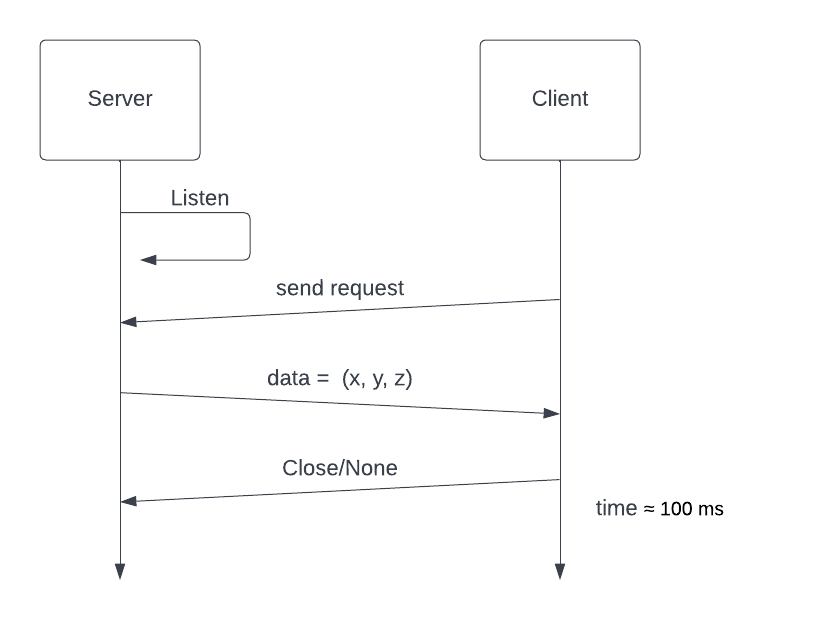
\includegraphics[scale=0.9]{chart_protokol}
\end{figure}

\section{Popis vybraných  nástrojů pro řešení}

\subsection{Python}

Jazyk použitý pro implementaci protokolu je Python. Zvolili jsme si tento jazyk z několika důvodů. 
Python má širokou standardní knihovnu, která obsahuje řadu modulů pro sítě a komunikaci, například sokety, které usnadňují vytvoření Protokolu.
Python má čistou a čitelnou syntaxi, která usnadňuje psaní a pochopení kódu. Navíc je to dynamicky typovaný jazyk, což znamená, že v kódu nemusíte uvádět typy proměnných. To může výrazně usnadnit psaní a debug kódu.
To je několik důvodů, proč byl vybrán oproti ostatním jazykům, jako například C, C++, Java a Go.\cite{python}

\subsection{MicroPython}

Dalším využitým nástrojem je MicroPython. MicroPython je implementace Pythonu, která je navržena pro snadné použití a provoz na malých mikrokontrolérech, jako ESP8266, ESP32 a Raspberry Pi Pico W. Tohoto dokázala díky speciální optimalizaci, která spočívá ve vymázání většiny standardní knihovny a přidání modulů pro specifickou práci s mikrokontroléry. Mezi tyto moduly patří moduly pro podporu sítí, interakci se senzory, displeji a dalšími hardwarovými komponentami.\cite{micropython}

\subsection{Raspberry Pi Pico W }

Hardwarové řešení je Raspberry Pi Pico W, která se hodí pro vytváření prototypů a experimentování. Snadno se používá a lze ji programovat v různých jazycích, včetně jazyků MicroPython a C. Díky tomu je skvělou volbou pro projekty, v nichž chcete rychle a snadno vytvářet prototypy a testovat své nápady. Dále má vestavěné rádio 2,4 GHz, které lze použít pro komunikaci WiFi, a na připojení Bluetooth Low Energy (BLE). Má i řadu digitálních a analogových vstupů a výstupů, které lze využít k propojení se senzory a dalšími zařízeními. Podporuje protokol I2C\footnote{Inter-Integrated Circuit}, který je důležitý pro práci s akcelometrem.  \cite{raspberry}

\begin{figure}[h]
\caption{Raspberry Pi Pico W}
\centering
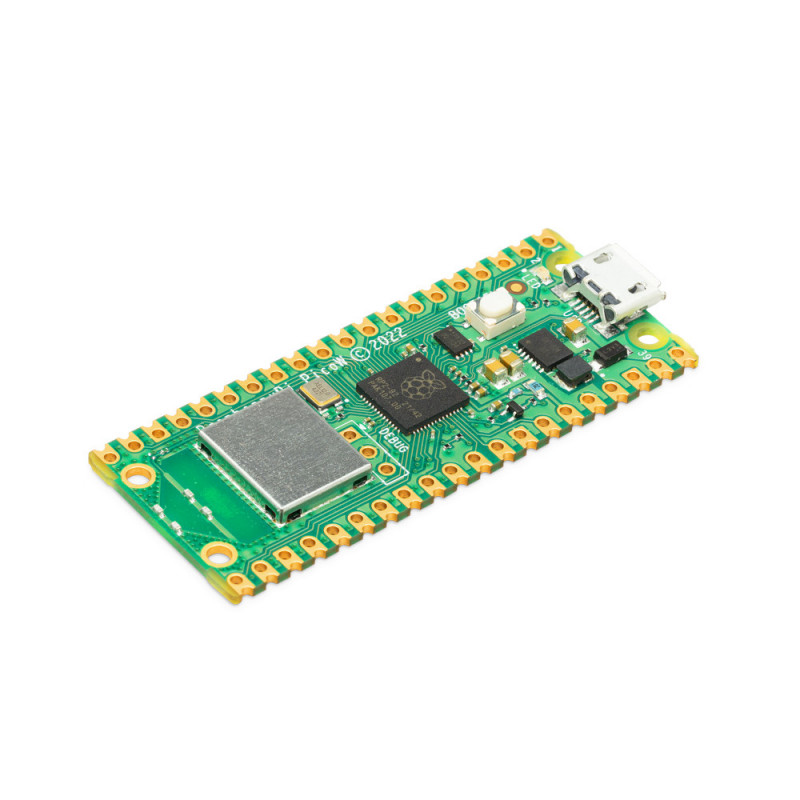
\includegraphics[scale=0.3]{raspberry}
\end{figure}

\subsection{Tříosý akcelerometr GY-291 s ADXL345}

Jako data pro přenos jsme vybrali data z
tříosého akcelerometru GY-291 s ADXL345. Tento senzor je přesný, cenově dostupný a používá se k měření pohybu a orientace. Měření probíhá ve 3 osách X, Y a Z a měří zrychlení v rozmezí -16 g až +16 g. Měření lze snadno získat, díky připojení akcelerometru GY-291 k mikrokontroléru pomocí rozhraní I2C. Tento senzor je kompatibilní s mikrokontroléry, jako je Arduino, Raspberry Pi a mnoho dalších.
\\
Senzor je také schopen detekovat orientaci v prostoru díky integrovanému gyroskopu. Jeho nejčastější použití spočívá v úkolech, jako stabilizace kamery nebo detekce pohybu v prostoru pro různé aplikace.
\\
Další možností pro sběr dat byl například senzor MPU-6050
, který má sběrnici dat v 6 rozměrech, ten kombinuje akcelometr v 3 osách a gyroskop také ve třech osách. Je určen na velmi přesné měření, které zde nebylo nutné. Další volbou byl senzor BNO055
 ten kombinuje akcelometr, gyroskop a magnetometr ve 3 osách, ten je určen na přesnou orientaci v prostoru, které také nebyla nutná. \cite{gyroskop}, \cite{MPU}, \cite{BNO}

\begin{figure}[h]
\caption{Tříosý akcelerometr GY-291 s ADXL345}
\centering
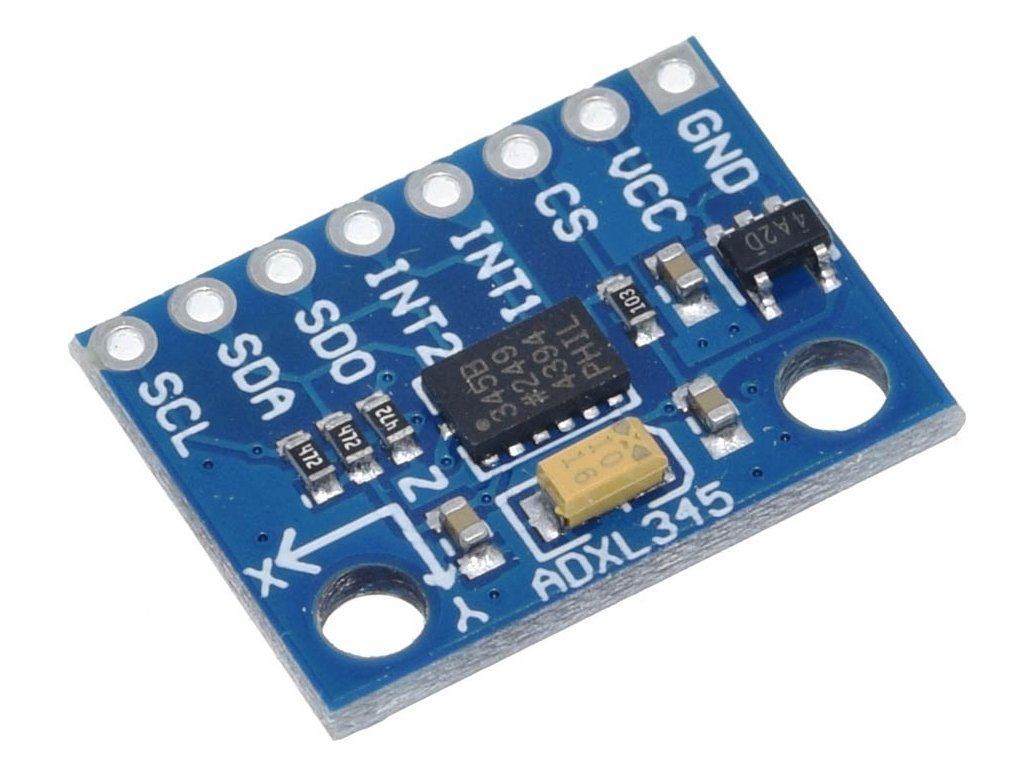
\includegraphics[scale=0.3]{gyroskop}
\end{figure}

\subsection{Modul \texttt{socket}}

Modul \texttt{socket} je vestavěný modul do jazyka Python, který poskytuje rozhraní pro práci se sockety, včetně jejich vytváření a používaní pro přijímání a odesílání dat po síti. Podporuje různé rodiny adres včetně \texttt{AF\_INET (IPv4)} a \texttt{AF\_INET6} (IPv6). Podporuje také řadu typů soketů, včetně \texttt{SOCK\_STREAM} (TCP) a \texttt{SOCK\_DGRAM} (UDP). \cite{socket}
\\
Díky tomuto modulu lze provádět spousty standardních akcí očekávaných od sítí, například navazovat spojení se servery, odesílat a přijímat data a uzavírat spojení, pokud již nejsou potřeba. 
\\
Alternativy k tomuto modulu jsou moduly 
\texttt{AsyncIO} a 
\texttt{PySocket}
. \texttt{AsyncIO} je standardní knihovna určena na asynchronní programování a mimo to podporuje i užití asynchroních socketů. Tato knihovna je vhodná pro aplikace vyžadující vysoký výkon a škálovatelnost. Tato knihovna nebyla vybrána z důvodu neznalosti asynchroního programování. \texttt{PySocket}, je modul třetí strany, který funguje na bázi \texttt{socket} modulu, jedná se pouze o jeho zjednodušení. \texttt{PySocket} nebyl vybrán z toho důvodu, že není implementován v MicroPythonu a není to standardní knihovna v Pythonu. \cite{async}, \cite{pysocket}

\subsection{Modul \texttt{network}}

Modul \texttt{network} je jeden z klíčových modulů v MicroPythonu, je určen pro možnost připojit se, odesílat zprávy a přijímat data přes síť. Poskytuje celou řadu síťových možností, konkrétně v protokolu je využit na připojení se k síti. \cite{network}

\subsection{Modul \texttt{json}}
Modul \texttt{json} je vestavěný modul v jazyce Python a  implementaci MicroPython. Poskytuje funkce pro práci s daty ve formátu JSON. Díky \texttt{json} knihovně je možné převádět data JSON na objekty jazyka Python a naopak. Jeho funkce umožňují jednoduchou serializaci dat a odeslání přes sockety \cite{json}
\\
Alternativou ke knihovně \texttt{json} je modul \texttt{ujson}. Tento modul je napsán v Pythonu a poskytuje rychlejší služby za využití méně paměti. Pro náš protokol, který je určen pro přenos malých dat, toto nebylo nutné. \cite{ujson}

\subsection{Moduly \texttt{machine} a \texttt{ADXL345}}
Modul \texttt{machine} je vestavěná knihovna v MicroPythonu určená pro práci s hardwarovými obvody, jako jsou časovače, I/O\footnote{input/output} piny a I2C rozhraní, které je podstatné pro práci s GY-291 s ADXL345. Tohoto modulu dále využívá modul třetí strany \cite{machine}

\texttt{ADXL345}, ten je užitečný pro snadnou práci s ADXL345. Modul získává z paměti informace o stavu zařízení a data naformátuje do stavu použitelného v aplikacích. K modulu \texttt{machine} existuje alternativa modul \texttt{pyb}, ten ale musí být doinstalován do MicroPythonu. K \texttt{ADXL345} modulu v momentu implementace nebyla alternativa. \cite{pyb}, \cite{adxl}


\subsection{Modul \texttt{random}}
\texttt{random} je vestavěná Python knihovna, ta umožňuje generovat pseudo náhodná čísla a provádět náhodné výběry. Nejvíce uplatnění tento modul najde při tvorbě her, či dalších programů, kde je potřeba generovat pseudo náhodné výsledky. \cite{random}
\\
Alternativou k modulu \texttt{random} je modul
 \texttt{secrets}
 . \texttt{Secretes} je modul, určený hlavně na generování kryptograficky bezpečných čísel a řetězců, což není nutné pro tvorbu videoher. \cite{secretes}
 
 
\subsection{Modul \texttt{pygame}}
\texttt{pygame} je sbírka různých Python modulů. Dohromady tvoří jeden celek, který je určen ke tvorbě videoher. Uživatel má možnost zobrazovat obraz, pouštět zvuk, či pracovat s uživatelským vstupem. Díky těmto možnostem můžete tvořit celé hry v Pythonu. \cite{pygame}
\\
\texttt{pygame} dále vyčnívá díky své dobré implementaci, kde hlavní funkce jsou tvořeny v jazyce C a Assembly. Tato implementace zaručuje dostatečnou rychlost kodů, která je při hrách nutná. Na to navazuje i snadná práce s více jádry najednou. Dále je pygame určen pro mnoho operačních systémů a mnoho prostředí. Toto vše z něj činí dobrý multifunkční nástroj, který je snadno přenositelný. 
\\
Další výhodou modulu \texttt{pygame} je důraz na jednoduchost použití a ovládání. Potřebná doba pro naučení se práci s ním je nízká, proto je velmi vhodný k testování protokolů.  
\\
Alternativa k \texttt{pygame} je například \texttt{pyglet}. \texttt{pyglet} je knihovna určená na práci se zobrazením oken a hraním zvuku. Na rozdíl od \texttt{pygame} má menší podporu pro vytváření videoher. Dalším důležitým rozdílem je, že \texttt{pyglet} používá jiný program pro vykreslování grafiky, ten je určen spíše pro 3D grafiku. \cite{pygame}, \cite{pyglet}

\subsection{Modul \texttt{multiprocessing}}
Modul \texttt{multiprocessing} je Python modul určený pro paralelní provádění kódů na několika jádrech. Umožňuje vytvářet několik samostatných procesů, které mohou běžet současně na jednom zařízení, či dokonce na několika síťově připojených počítačích. Tato funkce je užitečná pro výpočetně náročné úkoly a pro programy, kde je nutné, aby několik programů běželo ve stejnou chvíli. K tomu \texttt{multiprocessing} přidává možnosti sdílet data mezi těmito programy pomocí různých datových typů. \cite{multiprocess}
\\
Alternativa k modulu \texttt{multiprocessing} je modul \texttt{threading}. Hlavní rodíl mezi nimi je, že \texttt{threading} používá threads a \texttt{multiprocessing} používá procesy\footnote{proces je instance vytvořená multiprocessing modulem}. Ty se liší tím, že threads používají jedno jádro a procesy využívají více jader. Z toho vyplývají rozdíly ve funkčnosti. U procesů je náročné sdílet data, ale v případě chyby se ukončí pouze jeden proces a ne celý program. V případě chybovosti u threadu se ukončí celý program. Problém se sdílením dat je ale snadno řešitelný, díky implementaci modulu \texttt{multiprocessing}, a je tak vhodný pro můj protokol. \cite{threading}


\section{Popis řešení}
\subsection{Server}
Zdrojový kód pro server \ref{lst:server} je celý napsán v MicroPythonu. Kód začíná importem modulů, které jsou popsány v předešlé kapitole. Pokračujeme nastavením proměnných užitých později v programu. Proměnná \texttt{HOST} je využita na nastevení rozsahu, ve kterém bude server přijímat dotazy od klienta. Proměnná \texttt{PORT} je využita na nastavení portu, na kterém se server bude pohybovat. Nakonec zavedeme funkci pro připojení k internetu.
\begin{lstlisting}[title={Program server.py}, caption={server.py}, language=Python]
import socket
import network
from machine import Pin, I2C, SoftI2C
import ADXL345  # https://github.com/DFRobot/micropython-dflib/tree/master/ADXL345
from json import dumps

PORT = 8880
HOST = "0.0.0.0"

def do_connect(ssid, password):
    import network
    wlan = network.WLAN(network.STA_IF)
    wlan.active(True)
    if not wlan.isconnected():
        print('Connecting to network...')
        wlan.connect(ssid, password)
        while not wlan.isconnected():
            pass
    print(f'Network config: {wlan.ifconfig()}')

\end{lstlisting}
Nyní si zavedeme hlavní část programu, pro který jsme vytvořili blokové schéma pro jeho lepší pochopení. 

\begin{figure}[h]
\caption{blokový diagram serveru}
\centering
 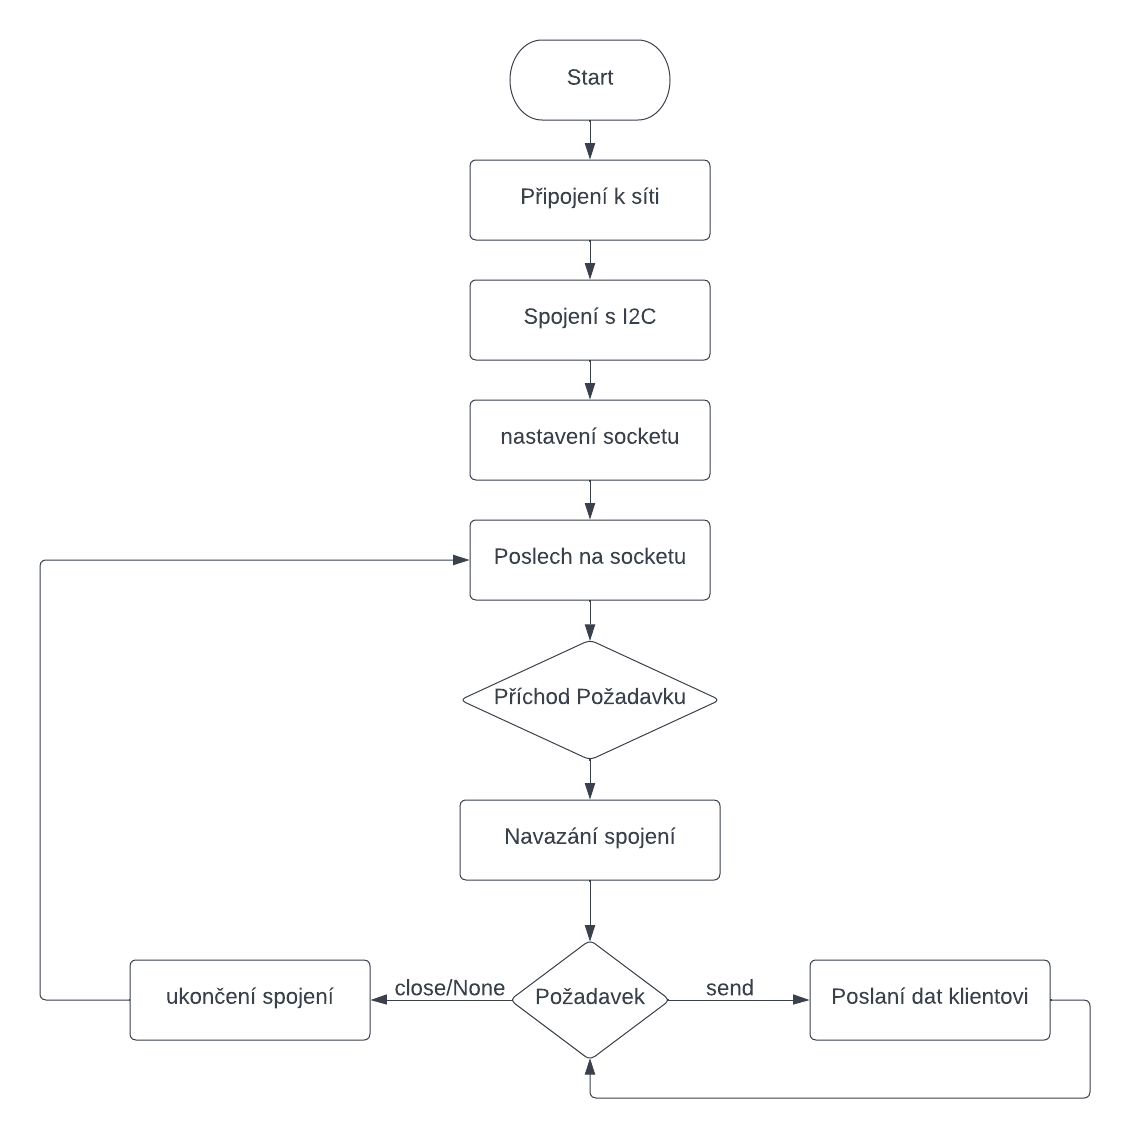
\includegraphics[scale=0.7]{block_scheme_server}
\end{figure}

Jak je vidět na schématu, nejdříve navážeme spojení se sítí díky funkci \texttt{do\_connect}. Pokračujeme vytvořením objektu \texttt{i2c}, předáme ho objektu \texttt{ADXL345}, díky kterému později budeme získávat souřadnice. Nakonec pokračujeme vytvořením socketu, v něm nastavíme typ protokolu. Na síťové vrstvě protokol IP a na transportní vrstvě protokol TCP. Dále nastavíme socketu jeho port číslo a rozmezí, na němž bude přijímat dotazy. Nakonec nastavíme, aby daný program poslouchal a bral maximálně 100 clientů v jeden moment. 

\begin{lstlisting}[title={Program server.py}, caption={server.py}, language=Python]
if __name__ == '__main__':
    do_connect("SSID", "password")
    i2c = SoftI2C(scl=Pin(17), sda=Pin(16), freq=10000)
    adx = ADXL345.ADXL345(i2c)
    soc = socket.socket(socket.AF_INET, socket.SOCK_STREAM)
    soc.setsockopt(socket.SOL_SOCKET, socket.SO_REUSEADDR, 1)
    soc.bind((HOST, PORT))
    soc.listen(100)
\end{lstlisting}

Nyní pokračujeme hlavní programovou smyčkou, tato smyčka je nekonečná. Ta čeká na dotaz klienta. Když se client dotáže, program spustí další smyčku. V té program přijme data poslané od klienta a dekóduje je. A nyní podle typu dat se rozhodne, jaký bude další postup. Pokud nejsou žádná data, nebo dávají dotaz na \texttt{close}, program uzavře spojení a nastaví socket tak, aby v případě nutnosti mohl být použit co nejdříve znovu. Když data dávají dotaz na \texttt{send}, program díky objektu \texttt{ADXL345} zjistí souřadnice akcelometru. Tyto data dá do datové struktury \texttt{tuple} a datovou strukturu serializuje způsobem JSON. Dále stejná data dá do kódování \texttt{UTF-8} a pošle je přes socket clientovi. 

\begin{lstlisting}[title={Program server.py}, caption={server.py}, language=Python]
  while True:
        print("wating for request")
        conn, address = soc.accept()
        while True:
            data = conn.recv(2048)
            data = data.decode("utf-8")
            print(data)
            if data == None:
                conn.close()
                soc.setsockopt(socket.SOL_SOCKET, socket.SO_REUSEADDR, 1)
                break
            if data == "send":
                x = adx.xValue
                y = adx.yValue
                z = adx.zValue
                data = dumps((x, y, z))
                conn.sendall(data.encode("utf-8"))
            elif data == "close":
                print("close")
                conn.close()
                soc.setsockopt(socket.SOL_SOCKET, socket.SO_REUSEADDR, 1)
                break
\end{lstlisting}

\subsection{Client}

Celý zdrojový kód klienta \ref{lst:client} je napsán v Pythonu. Kód začína importem modulů a pokračuje stanovením globálních proměnných. Nastaví proměnné \texttt{PORT} a \texttt{IP}, ty musí souhlasit s nastavením serveru. 
\begin{lstlisting}[title={Program client.py}, caption={client.py}, language=Python]
import socket
from json import loads

PORT = 8880
IP = "192.168.102.197"
\end{lstlisting}

Nyní se zaměříme na hlavní kód programu, je napsán ve funkci z důvodu jeho pozdějšího použití, jako proces. Zároveň má jeden argument \texttt{queue}, to je objekt modulu \texttt{multiprocessing}, ten je později využit na sdílení dat mezi procesy. Pokračujeme hlavním programem. Nejdříve nastavíme typ protokolu. Na síťové vrstvě protokol IP a na transportní vrstvě protokol TCP. 


\begin{figure}[h]
\caption{blokový diagram clienta}
\centering
 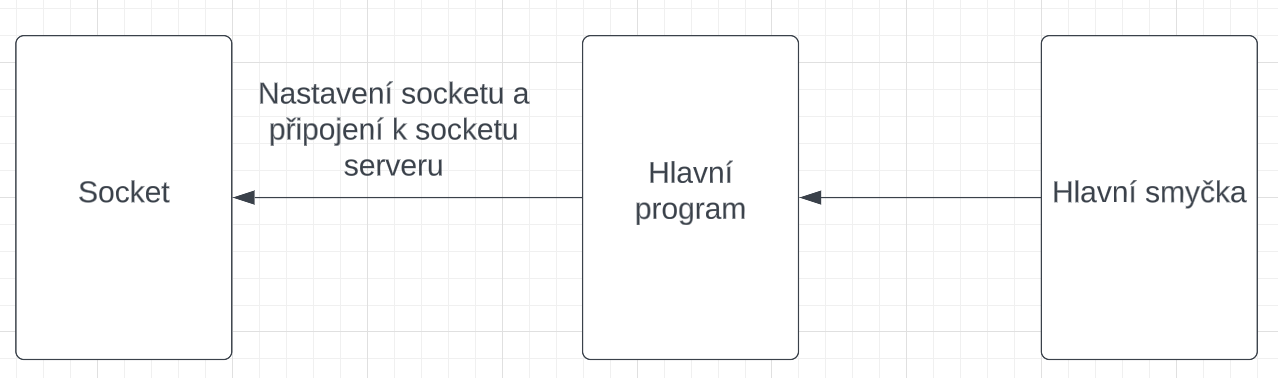
\includegraphics[scale=0.8]{block_scheme_client}
\end{figure}

Dále definujeme hlavní smyčku. Ta se ihned po spuštění dostane do další smyčky. V této smyčce se nejdříve serveru pošle požadavek na \texttt{send}. Dále klient vyzkouší, jestli mu server poslal data. V případě že data nejsou přijata, vydá se chybové hlášení o ztracení kontatku a klient se pokusí znovu navázat kontakt. Jestli jsou data přijata, klient je dekóduje. Přeformátuje je z JSON formátu do formátu datové struktury \texttt{tuple}. Dále tyto data vloží do řady. Toto opakuje do té doby, než se program přeruší. 

\begin{lstlisting}[title={Program client.py}, caption={client.py}, language=Python]
def client(queue):
    s = socket.socket(socket.AF_INET, socket.SOCK_STREAM)
    s.connect((IP, PORT))
    while True:
        print("Sending")
        while True:
            msg = "send"
            s.sendall(msg.encode("utf-8"))
            try:
                data = s.recv(1024)
            except socket.error:
                print("Connection lost")
                continue
            data = data.decode("utf-8")
            data = loads(data)
            queue.put(data)

\end{lstlisting}

\subsection{Diskuze řešení}
Výsledek je funkční a je proveden pomocí zamýšlené implementace. Toto umožní uživateli, který vlastní zařízení Raspberry Pi Pico W s ADXL345, účinně přenášet data o poloze přes WiFi, k různým účelům. 
\\
Limitací ze strany serveru je několik.
 Program umožňuje pouze dva typy dotazů a to \texttt{send} a \texttt{close}. Proto může dojít k tomu, že klient pošle jiný dotaz, a s tímto dotazem nemusí být naloženo adekvátně. Dále kód nemá implementované žádné mechanismy proti chybám, nebude proto přiraven na selhání, popřípadě na různé krajní situace. Následně i přestože je komunikace pouze v lokální síti, měla by být šifrována. Dalším úzkalím může být, že kód není optimalizován na výkonnost, či práci s pamětí. Pokud tedy uživatel bude chtít použít zařízení s menší výkonností nežli Raspberry Pi Pico W, může se dostat do problémů. A v poslední řadě, server může pracovat pouze s akcelerometrem ADXL345 a nepodporuje jiné modely akcelerometrů.
\\
Limitací ze stran klienta je také několik. Jedním z hlavních omezení je, že program pracuje pouze s jednou přednastavenou IP adresou, optimálnější by bylo, kdyby ji bylo možné určit dynamicky. Dalším problémem je, že klient není připraven na případné chyby, proto může snadno dojít k jeho selhání. Důkazem toho je předpoklad klienta, že server je spuštěný, pokud by nebyl, klient automaticky selže. Nakonec, klient po obdržení dat neodešle serveru žádnou potvrzovací zprávu, takže server neví, zda klient data úspěšně přijal. 
\\
Další směr vývoje může spočívat nejdříve v implementaci systému proti chybáma a selháním a uskutečnění šifrování. Následný vývoj může spočívat ve vytvoření automatického nastavení IP adresy serveru, tak aby to  více vyhovovalo klientské straně. Konečný vývoj by umožňoval využití co nejširšího počtu zařízení. Toho se dá dosáhnout vytvořením serveru tak, aby podporoval co nejvíce zařízení. 

\section{Využití dat}
\subsection{Návrh videohry}
Pro ukázku praktického využití dat jsme si vybrali projekt založený na vytvoření videohry. Základní princip hry spočívá ve vesmírné lodi, která se vyhýbá meteoritům, a zároveň se snaží sbírat mince. Uživatel pohybuje s Raspberry Pi Pico W s ADXL345, pomocí toho ovládá loď na obrazovce a snaží se vyhýbat meteoritům. Po každém zásahu vemírné lodi meteoritem, se hráči ubere jeden život. Zároveň se hráči počítá skóre, které se zvyšuje sběrem mincí.
 
\subsection{Popis videohry}
Hráč se nejdříve objeví na hlavní obrazovce. Odtud má dvě možnosti. Může se podívat na celkové nejlepší skóre, které kdy nahrál. Další možnost je spustit hru. Po spuštění hry se objeví na obrazovce, kde se na dolní liště pohybuje vesmírná loď. Ta kopíruje pohyby hráče se zařízením na ovládání. Ihned po spuštění se na horní listě také objeví meteority a mince, které putují k dolní liště, pod náhodným sklonem s náhodnou rychlostí. Dále se v levém horním rohu objeví celkový počet získaných mincí. V pravém horním rohu se ukazují obrázky ve tvaru srdce, které znázorňují životy hráče. Po každém nárazu hráče do meteoritu jedno srdce změní barvu na šedou, tím signalizuje ztrátu jednoho života. Životy jsou celkem tři. 


\subsection{Popis řešení videohry}
Po spuštění se program rozdělí do dvou procesů. A to proces, ve kterém se nachází hra a proces klienta. 

\begin{lstlisting}[title={Program game.py}, caption={game.py}, language=Python]
if __name__ == "__main__":
    queue = Queue() 
    menu_proc = Process(target=main_menu, args=(queue,)) 
    client_proc = Process(target=client, args=(queue,))  
    client_proc.start()
    menu_proc.start()
    client_proc.join()
    menu_proc.join()
\end{lstlisting}

Hra se dále dělí na několik funkcí, kde každá znázorňuje jednu obrazovku. Konkrétně jsou tři obrazovky, a to obrazovka se skóre, hlavní obrazovka a obrazovka videohry.
\\
Klient se mezitím spojí se serverem a začne generovat data. Oba tyto procesy mezitím sdílejí obejkt \texttt{queue}, který značí řadu. Do tohoto objektu klient přidává data získané od serveru, a jelikož proces se hrou běží 60-krát za sekundu, tak ihned data vyjme ze řady a použije je pro ovládání vesmírné lodi. Druhá možnost je, že data vyjme z řady a zahodí je, aby se loď nezačala pohybovat náhodně, pokud hráč znovu spustí hru.


\begin{figure}[h]
\caption{blokový diagram videohry}
\centering
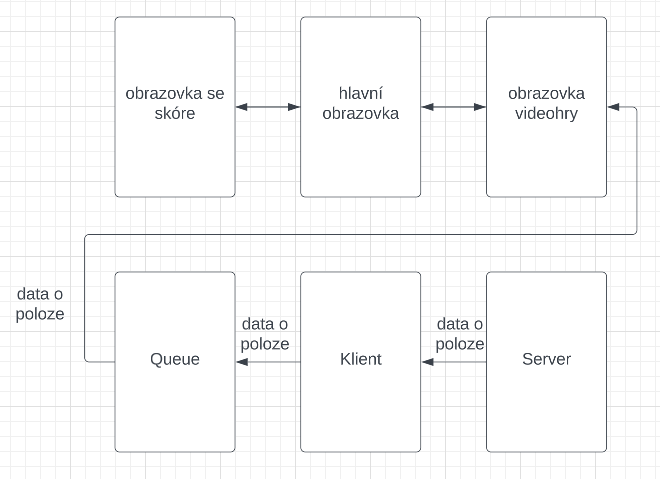
\includegraphics[scale=0.9]{game_diagram}
\end{figure}

Nyní se dostáváme k herní logice. Ta se celá nachází v obrazovce s videohrou, konkrétně v její smyčce, která probíhá 60-krát za sekundu. Kvůli této rychlosti, se program nejdříve podívá, jestli objekt \texttt{queue} není prázdný. Pokud je prázdný, program pokračuje. Pakliže je v ní nějaký prvek, program vyjme data z řady a začne vypočítávat rychlost. 
To konkrétně pomocí změny proměnné s názvem \texttt{ship\_speed}. Jestli se uživatel dostane za hranici levé lišty, program začne lodi přidávat takovou hodnotu, aby loď pokračovala na pravou stranu a naopak. Toto je napsáno proto, aby se loď nezasekla na žádné z bočních stran. Dále program zkontroluje velikost dat, 
a to konkrétně, jestli data jdou do záporných, či kladných hodnot. Jestliže jsou hodnoty záporné, loď se začne pohybovat levým směrem a naopak. Hodnota rychlosti se dále vypočítává pomocí lineární funkce, a to z toho důvodu, aby ovladač měl větší citlivost na prudké pohyby ovladačem, či naopak jemné pohyby. 



\begin{lstlisting}[title={Program game.py}, caption={game.py}, language=Python]
if queue.empty() is False:
	data = queue.get()
    print(data)
    if ship_rect.left > W: 
        ship_speed -= 2
    elif ship_rect.left < 0:  
        ship_speed += 2
    elif data[2] > 0:
        ship_speed += 0.01 * data[2] 
    elif data[2] <= 0:
        ship_speed += 0.01 * data[2]

\end{lstlisting}


Dále začneme využívat rychlost lodi. Nejdříve znovu zkontrolujeme, že loď není mimo obrazovku, pokud loď mimo obrazovku je, tak její rychlost nastavíme na nula. Tím zamezíme možnosti vyjetí lodi 
mimo obrazovku. Nyní přičteme k objektu vesírmé lodi vypočítanou rychlost a pokračujeme v dalším doladění pohybu. Prvně když chtěl hráč rychle změnit směr pohybu lodi, tak se pohybovala pomalu, jelikož se rychlost nasčítávala. Pro tento problém jsme zavedli následné řešení. Nejdříve zkontrolujeme jestli stará pozice byla záporná, a pokud zároveň byla nynější rychlost kladná, tak rychlost vynulujeme. Tím může loď ostře změnit svůj směr, a to i obráceně. Dále jestli rychlost lodi, kvůli nasčítaní byla moc veliká tak program rychlost zmenší, aby byla snadněji ovladatelná. 



\begin{lstlisting}[title={Program game.py}, caption={game.py}, language=Python]
if 0 <= ship_rect.left + ship_speed <= W - 90: 
    ship_rect.left += ship_speed
    if old_position < 0 < ship_speed:  
        ship_speed -= ship_speed
    elif old_position > 0 > ship_speed:  
        ship_speed += ship_speed
    if ship_speed > 200:  
        ship_speed -= 100
else:
    ship_speed = 0

\end{lstlisting}


\subsection{Diskuze videohry}

Videohra dává bližší důkaz o reálném použití dat pro různé aplikace. Je možné díky ní si přiblížit odezvu protokolu a jeho schopností. 
\\
Ačkoli hra slouží jako užitečný nástroj, má určitá omezení. Hlavním omezením je její implementace, zejména pokud jde o logiku použitou pro výpočet rychlosti kosmické lodi. Ta by mohla být zlepšena, aby se zvýšila její citlivost a celková uživatelská přívětivost. Kromě toho se objevuje problém s pohybem ostatních objektů ve hře, ty mají tendenci opakovat určité pohyby nebo se nesrazí se spodní částí obrazovky.
\\
Pro zlepšení hratelnosti by se budoucí vývoj mohl zaměřit na zdokonalení logiky pohybu vesmírné lodi a současně řešit pohyb ostatních objektů ve hře. Je však důležité poznamenat, že protokol má potenciální využití i mimo hru, například v robotice nebo při řízení stability a detekci pádů.



	\chapter*{Závěr}
	
		V této práci jsme se zabývali základy komunikace na úrovni TCP/IP a zaměřili jsme se na praktické aplikace protokolu TCP (Transmission Control Protocol). Nejdříve jsme rozebrali, jakým způsobem zařízení komunikují, a dále protokoly, které jim toto usnadňují. Popsali jsme návrh a vývoj vlastního aplikačního protokolu založeného na rodině protokolů TCP/IP s cílem usnadnit komunikaci mezi mikropočítačem a osobním počítačem. Poté jsme demonstrovali funkčnost tohoto protokolu v reálném scénáři pomocí mikropočítače a osobního počítače.
\\
Prostřednictvím naší praktické implementace jsme byli schopni vyhodnotit navrhovaný protokol a určit jeho silné stránky a omezení. Zjistili jsme, že protokol je schopen efektivně navázat a udržovat komunikaci mezi oběma zařízeními s minimálním zpožděním. Zaznamenali jsme však také, že by bylo možné provést další zlepšení. Hlavně co se týče odolnosti systému proti chybám a jeho zabezpečení.  
\\
S ohledem na tato zjištění navrhujeme, aby se budoucí výzkum v této oblasti zaměřil na odstranění zjištěných omezení, konkrétně v oblasti bezpečnosti a dynamičnosti protokolu. Kromě toho by bylo vhodné prozkoumat využití tohoto protokolu v dalších komunikačních scénářích, například v robotice, či při detekci pádů.
\\
Celkově tato práce přispěla k pochopení protokolu TCP a jeho praktickému využití v konkrétním komunikačním scénáři. Doufáme, že poslouží jako cenný zdroj informací pro studenty a odborníky z praxe, kteří se zajímají o protokoly TCP, a že bude inspirací pro další výzkum v této oblasti.
	
	\nocite{*}
    	\printbibliography					
	\addcontentsline{toc}{chapter}{Bibliografie}
    \printglossary[title={Zkratky}]		
    \listoffigures					
						

    \begin{appendices}
	\chapter{Zdrojový kód serveru}
	
\begin{lstlisting}[title={Program server.py}, caption={server.py},  label={lst:server}, language=Python]


import socket
import network
from machine import Pin, I2C, SoftI2C
import ADXL345  # https://github.com/DFRobot/micropython-dflib/tree/master/ADXL345
from json import dumps

PORT = 8880
HOST = "0.0.0.0"


def do_connect(ssid, password):
    import network
    wlan = network.WLAN(network.STA_IF)
    wlan.active(True)
    if not wlan.isconnected():
        print('Connecting to network...')
        wlan.connect(ssid, password)
        while not wlan.isconnected():
            pass
    print(f'Network config: {wlan.ifconfig()}')


if __name__ == '__main__':
    do_connect("SSID", "password")
    i2c = SoftI2C(scl=Pin(17), sda=Pin(16), freq=10000)
    adx = ADXL345.ADXL345(i2c)
    soc = socket.socket(socket.AF_INET, socket.SOCK_STREAM)
    soc.setsockopt(socket.SOL_SOCKET, socket.SO_REUSEADDR, 1)
    soc.bind((HOST, PORT))
    soc.listen(100)
    while True:
        print("wating for request")
        conn, address = soc.accept()
        while True:
            data = conn.recv(2048)
            data = data.decode("utf-8")
            if data == None:
                conn.close()
                soc.setsockopt(socket.SOL_SOCKET, socket.SO_REUSEADDR, 1)
                break
            if data == "send":
                x = adx.xValue
                y = adx.yValue
                z = adx.zValue
                data = dumps((x, y, z))
                conn.sendall(data.encode("utf-8"))
            elif data == "close":
                print("close")
                conn.close()
                soc.setsockopt(socket.SOL_SOCKET, socket.SO_REUSEADDR, 1)
                break


\end{lstlisting}

	\chapter{Zdrojový kód clienta}

\begin{lstlisting}[title={Program client.py}, caption={client.py},  label={lst:client}, language=Python]

import socket
from json import loads

PORT = 8880
HOST = "0.0.0.0"
IP = "192.168.102.197"   #Default raspberry pi ip address

def client(queue):
    s = socket.socket(socket.AF_INET, socket.SOCK_STREAM)
    s.connect((IP, PORT))
    while True:
        print("Sending")
        while True:
            msg = "send"
            s.sendall(msg.encode("utf-8"))
            try:
                data = s.recv(1024)
            except socket.error:
                print("Connection lost")
                continue
            data = data.decode("utf-8")
            data = loads(data)
            queue.put(data)

\end{lstlisting}
	\chapter{Zdrojový kód videohry}
	
\begin{lstlisting}[title={Program hra.py}, caption={hra.py},  label={lst:hra}, language=Python]
"""
author = Alex Olivier Michaud
This is the main file of the game, it is used to start the game, show the score and exit the game.
The game is a space shooter like, where you have to avoid the asteroids
to navigate the ship it uses an accelerometer, connected to a raspberry pi
"""
# TODO: reunite the language of the code to english
import pygame
from sys import exit
from random import randint, uniform
from multiprocessing import Process, Queue
from client import client
import sqlite3

# Global variables for window size
H = 800
W = 1000

def score(queue):
    """
    This function is used to show the score in the menu of the game
    :param queue: the main queue of the game to share resources
    :return: None
    """
    global H, W
    pygame.init()
    screen = pygame.display.set_mode((W, H))
    # pygame.image.load("menu.png")
    myFont = pygame.font.Font("8-BIT WONDER.ttf", 30)
    pygame.display.update()
    # database of score
    conn = sqlite3.connect('score.db')
    c = conn.cursor()
    c.execute("CREATE TABLE IF NOT EXISTS score (score integer)")
    c.execute("""SELECT MAX(score) FROM score""")
    data = c.fetchone()
    print(data)
    conn.close()
    if data[0] is None:
        data = 0
    run = True
    while run:
        screen.blit(pygame.image.load("img/menu.png"), (-10, -90))
        # create text
        text_1 = myFont.render("Best Score", True, (0, 0, 0))
        text_2 = myFont.render("Return", True, (0, 0, 0))
        text_score = myFont.render(str(data[0]), True, (0, 0, 0))
        # Creating text rectangles
        text_1_rect = text_1.get_rect(midtop=(W / 2, 300))
        text_2_rect = text_2.get_rect(midtop=(W / 2, 400))
        text_score_rect = text_score.get_rect(midtop=(W / 2, 350))
        # blit text
        screen.blit(text_1, text_1_rect)
        screen.blit(text_2, text_2_rect)
        screen.blit(text_score, text_score_rect)
        for event in pygame.event.get():
            if event.type == pygame.QUIT:
                run = False
                queue.put("exit")
                exit()
            if event.type == pygame.MOUSEBUTTONDOWN:
                if text_2_rect.collidepoint(event.pos):
                    run = False
                    main_menu(queue)
        pygame.display.flip()
    return


def main_menu(queue):
    """
    This function is used to show the main menu of the game, which is used to start the game,
    show the score and exit the game
    :param queue: the main queue of the game to share resources
    :return: None
    """
    global H, W
    pygame.init()
    screen = pygame.display.set_mode((W, H))
    # font is from https://www.dafont.com/8bit-wonder.font
    myFont = pygame.font.Font("8-BIT WONDER.ttf", 30)
    pygame.display.update()
    run = True
    while run:
        # the queue is used here, because the client is always running, so if you restart the game,
        # the spaceship would otherwise move in a random direction, so if you empty the queue,
        # the spaceship will not move, until you move it, and the [0,0,0] is
        # here, so you will start the game with the spaceship in the middle of the screen
        queue.get()
        if queue.empty():
            queue.put([0, 0, 0])
        # create background
        screen.blit(pygame.image.load("img/menu.png"), (-10, -90))
        # create text
        text_1 = myFont.render("Avoid Asteroids", True, (0, 0, 0))
        text_2 = myFont.render("Press tab to start", True, (0, 0, 0))
        text_3 = myFont.render("Check the score", True, (0, 0, 0))
        # Creating text rectangles
        text_1_rect = text_1.get_rect(midtop=(W / 2, 300))
        text_2_rect = text_2.get_rect(midtop=(W / 2, 350))
        text_3_rect = text_3.get_rect(midtop=(W / 2, 400))
        # blit text
        screen.blit(text_1, text_1_rect)
        screen.blit(text_2, text_2_rect)
        screen.blit(text_3, text_3_rect)
        for event in pygame.event.get():
            if event.type == pygame.QUIT:
                run = False
                queue.put("exit")
                exit()
            if event.type == pygame.KEYDOWN:
                if event.key == pygame.K_SPACE:
                    run = False
                    App(queue)
            if event.type == pygame.MOUSEBUTTONDOWN:
                if text_2_rect.collidepoint(event.pos):
                    run = False
                    App(queue)
                if text_3_rect.collidepoint(event.pos):
                    run = False
                    score(queue)
        pygame.display.flip()


def App(queue):
    """
    This function is used to show the game, and to control the game
    :param queue:
    :return:
    """
    global H, W
    pygame.init()
    screen = pygame.display.set_mode((W, H))
    pygame.display.set_caption("Space Invaders")
    clock = pygame.time.Clock()
    font = pygame.font.SysFont("Arial", 30)

    # import images
    sky_surface = pygame.image.load("img/l.png")
    ship = pygame.image.load("img/ship.png").convert_alpha()
    meteorite = pygame.image.load("img/meteorite.png").convert_alpha()
    meteorite_2 = pygame.image.load("img/meteorite_2.png").convert_alpha()
    coin = pygame.image.load("img/coin.png").convert_alpha()
    heart = pygame.image.load("img/heart_for_game.png").convert_alpha()
    dead_heart = pygame.image.load("img/die_heart_game.png").convert_alpha()

    # scale images
    ship = pygame.transform.scale(ship, (90, 90))
    meteorite = pygame.transform.scale(meteorite, (90, 90))
    meteorite_2 = pygame.transform.scale(meteorite_2, (90, 90))
    coin = pygame.transform.scale(coin, (90, 90))
    heart = pygame.transform.scale(heart, (50, 50))
    dead_heart = pygame.transform.scale(dead_heart, (50, 50))

    # coordinates
    ship_x = 450
    meteorite_x = randint(0, 1000)
    meteorite_y = 0
    meteorite_x_2 = randint(0, 1000)
    meteorite_y_2 = 0
    coin_x = randint(0, 1000)
    coin_y = 0

    # rectangles
    ship_rect = ship.get_rect(midbottom=(ship_x, 800))
    meteorite_rect = meteorite.get_rect(midbottom=(meteorite_x, meteorite_y))
    meteorite_rect_2 = meteorite_2.get_rect(midbottom=(meteorite_x_2, meteorite_y_2))
    coin_rect = coin.get_rect(midbottom=(coin_x, coin_y))
    sky_surface_rect = sky_surface.get_rect(topleft=(0, 0))
    heart_rect = heart.get_rect(topright=(W, 0))
    heart_rect_2 = heart.get_rect(topright=(W - 50, 0))
    heart_rect_3 = heart.get_rect(topright=(W - 100, 0))
    dead_heart_rect = dead_heart.get_rect(topright=(W, 0))
    dead_heart_rect_2 = dead_heart.get_rect(topright=(W - 50, 0))
    dead_heart_rect_3 = dead_heart.get_rect(topright=(W - 100, 0))

    # speed
    ship_speed = 0
    meteorite_speed = 5
    meteorite_speed_2 = 5
    coin_speed = 5
    # speed in y
    meteorite_speed_y = 0
    meteorite_speed_y_2 = 0
    coin_speed_y = 0

    # number of coins
    coins = 0
    # number of lives
    lives = 3

    # text for coins
    coins_text = font.render(f"Coins: {coins}", True, (255, 255, 255))

    # previous position
    old_position = 0

    run = True
    while run:
        for event in pygame.event.get():
            if event.type == pygame.QUIT:
                queue.put("exit")
                pygame.quit()
                exit()

        # spawning objects
        screen.blit(sky_surface, (0, 0))
        screen.blit(ship, ship_rect)
        screen.blit(meteorite, meteorite_rect)
        screen.blit(meteorite_2, meteorite_rect_2)
        screen.blit(coin, coin_rect)
        screen.blit(coins_text, (10, 10))
        screen.blit(heart, heart_rect)
        screen.blit(heart, heart_rect_2)
        screen.blit(heart, heart_rect_3)

        # checking the number of lives and spawning dead hearts if needed
        if lives == 2:
            screen.blit(dead_heart, dead_heart_rect)
        if lives == 1:
            screen.blit(dead_heart, dead_heart_rect)
            screen.blit(dead_heart, dead_heart_rect_2)
        if lives == 0:
            screen.blit(dead_heart, dead_heart_rect)
            screen.blit(dead_heart, dead_heart_rect_2)
            screen.blit(dead_heart, dead_heart_rect_3)
            # updating the number of score in the database
            conn = sqlite3.connect("score.db")
            cursor = conn.cursor()
            cursor.execute("CREATE TABLE IF NOT EXISTS score (score integer)")
            cursor.execute("INSERT INTO score VALUES (?)", (coins,))
            conn.commit()
            conn.close()
            run = False
            ###game over###
            main_menu(queue)

        if queue.empty() is False:
            data = queue.get()
            print(data)
            if ship_rect.left > W:  # if the ship is out of the screen
                ship_speed -= 2
            elif ship_rect.left < 0:  # if the ship is out of the screen
                ship_speed += 2
            elif data[2] > 0:
                ship_speed += 0.01 * data[2]  # linear function to represent the speed of the ship
            elif data[2] <= 0:
                ship_speed += 0.01 * data[2]

        # TODO: make the ship movement more smooth
        if 0 <= ship_rect.left + ship_speed <= W - 90:  # if the ship is in the screen
            ship_rect.left += ship_speed
            if old_position < 0 < ship_speed:  # better movement, if the ship is moving to the right
                # it resets the speed, thus making the movement smoother
                ship_speed -= ship_speed
            elif old_position > 0 > ship_speed:  # same as above but for the left
                ship_speed += ship_speed
            if ship_speed > 200:  # if the speed is too high, it resets it
                ship_speed -= 100
        else:
            ship_speed = 0

        # moving objects, random sleep, random spawn, random speed
        if sky_surface_rect.colliderect(meteorite_rect) is False:
            if meteorite_rect.left == 0:  # if its 0 I would get a division by 0 error
                meteorite_rect.left = 1
            meteorite_speed_y = uniform(-1 * (1000 / meteorite_rect.left), 1000 / (
                    1000 - meteorite_rect.left))  # linear function to represent the direction of the meteorite
            meteorite_speed = randint(3, 10)  # random speed in x
            meteorite_rect.top = 0  # respawn the meteorite at the top of the screen

        if sky_surface_rect.colliderect(meteorite_rect_2) is False:
            if meteorite_rect_2.left == 0:  # if its 0 I would get a division by 0 error
                meteorite_rect_2.left = 1
            meteorite_speed_y_2 = uniform(-1 * (1000 / meteorite_rect_2.left), 1000 / (
                    1000 - meteorite_rect_2.left))  # linear function to represent the direction of the meteorite
            meteorite_speed_2 = randint(3, 10)  # random speed in x
            meteorite_rect_2.top = 0  # respawn the meteorite at the top of the screen

        if sky_surface_rect.colliderect(coin_rect) is False:
            if coin_rect.left == 0:  # if its 0 I would get a division by 0 error
                coin_rect.left = 1
            coin_speed_y = uniform(-1 * (1000 / coin_rect.left), 1000 / (
                    1000 - coin_rect.left))  # linear function to represent the direction of the meteorite
            coin_speed = randint(3, 10)  # random speed in x
            coin_rect.top = 0  # respawn the meteorite at the top of the screen

        # moving objects
        meteorite_rect.top += meteorite_speed
        meteorite_rect_2.top += meteorite_speed_2
        coin_rect.top += coin_speed
        # moving objects in y. m,
        meteorite_rect.left += meteorite_speed_y
        meteorite_rect_2.left += meteorite_speed_y_2
        coin_rect.left += coin_speed_y

        # collisions with the ship, if the ship collides with the meteorite, it loses a life
        # if the ship collides with the coin, it gets a coin and updates the score
        if meteorite_rect.colliderect(ship_rect):
            lives -= 1
            meteorite_rect.top = 0

        if meteorite_rect_2.colliderect(ship_rect):
            lives -= 1
            meteorite_rect_2.top = 0

        if coin_rect.colliderect(ship_rect):
            coins += 1
            coins_text = font.render(f"Coins: {coins}", True, (255, 255, 255))
            coin_rect.top = 0

        pygame.display.update()
        clock.tick(60)


if __name__ == "__main__":
    queue = Queue()  # object to communicate between the processes,
    # the queue is used for the data from the accelerometer the format is [x, y, z]
    menu_proc = Process(target=main_menu, args=(
        queue,))  # process for the menu, it interacts with the functions App() and Score(),
    # so these processes are not needed
    client_proc = Process(target=client, args=(
        queue,))  # process for the accelerometer, it sends the data to the queue,
    # it is imported from the client.py file
    client_proc.start()
    menu_proc.start()
    client_proc.join()
    menu_proc.join()
    ##TODO: if the process menu_proc is closed, the client_proc processes should be closed too

\end{lstlisting}
\begin{figure}[h]
\caption{hlavní obrazovka}
\centering

\includegraphics[scale=0.5]{1}
\end{figure}

\begin{figure}[h]
\caption{obrazovka videohry}
\centering
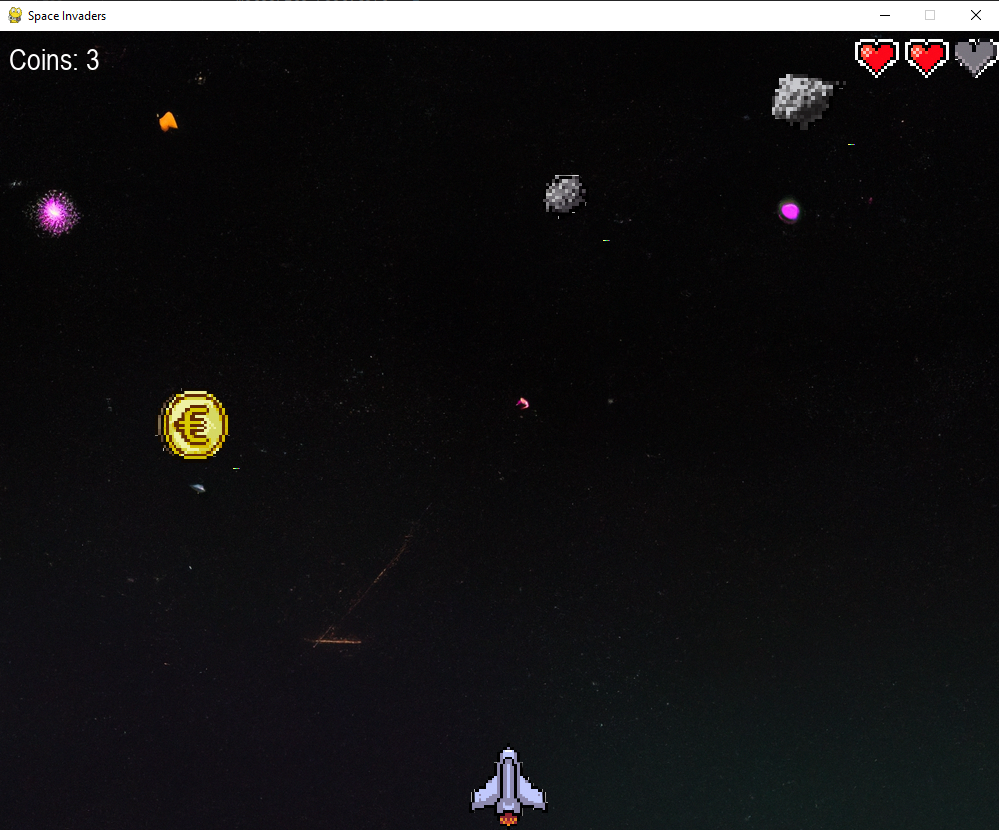
\includegraphics[scale=0.5]{2}
\end{figure}

\begin{figure}[h]
\caption{obrazovka skóre}
\centering
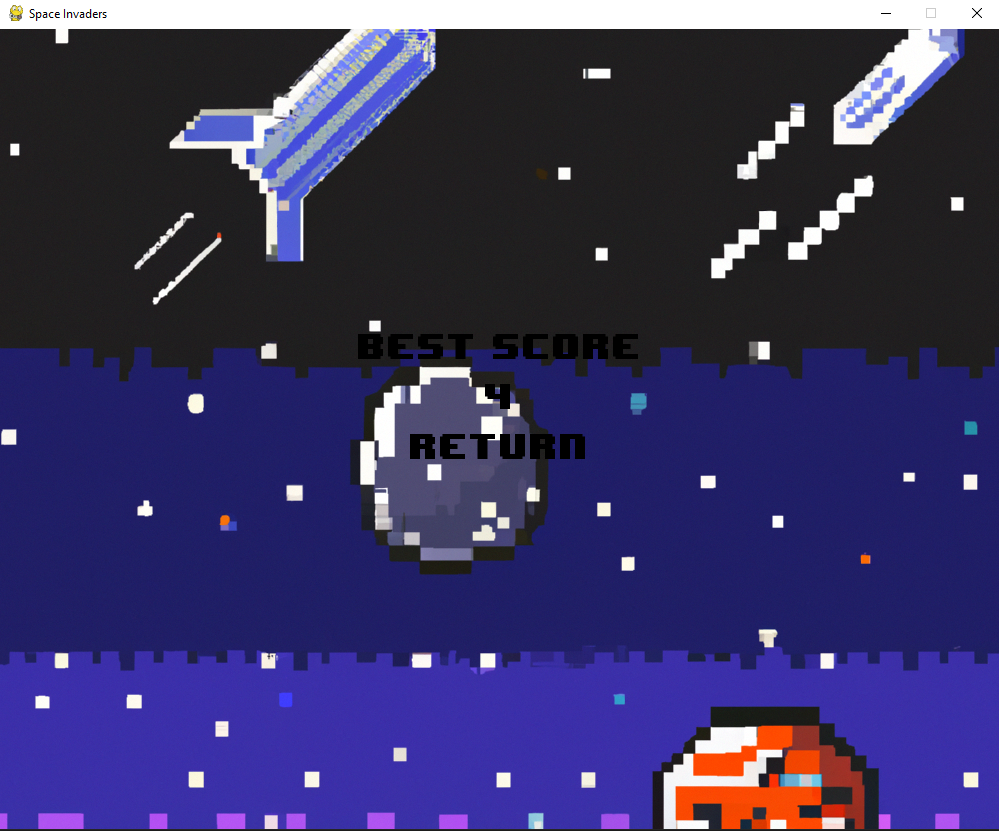
\includegraphics[scale=0.5]{3}
\end{figure}

\begin{figure}[h]
\caption{destička s Raspberry Pico W}
\centering
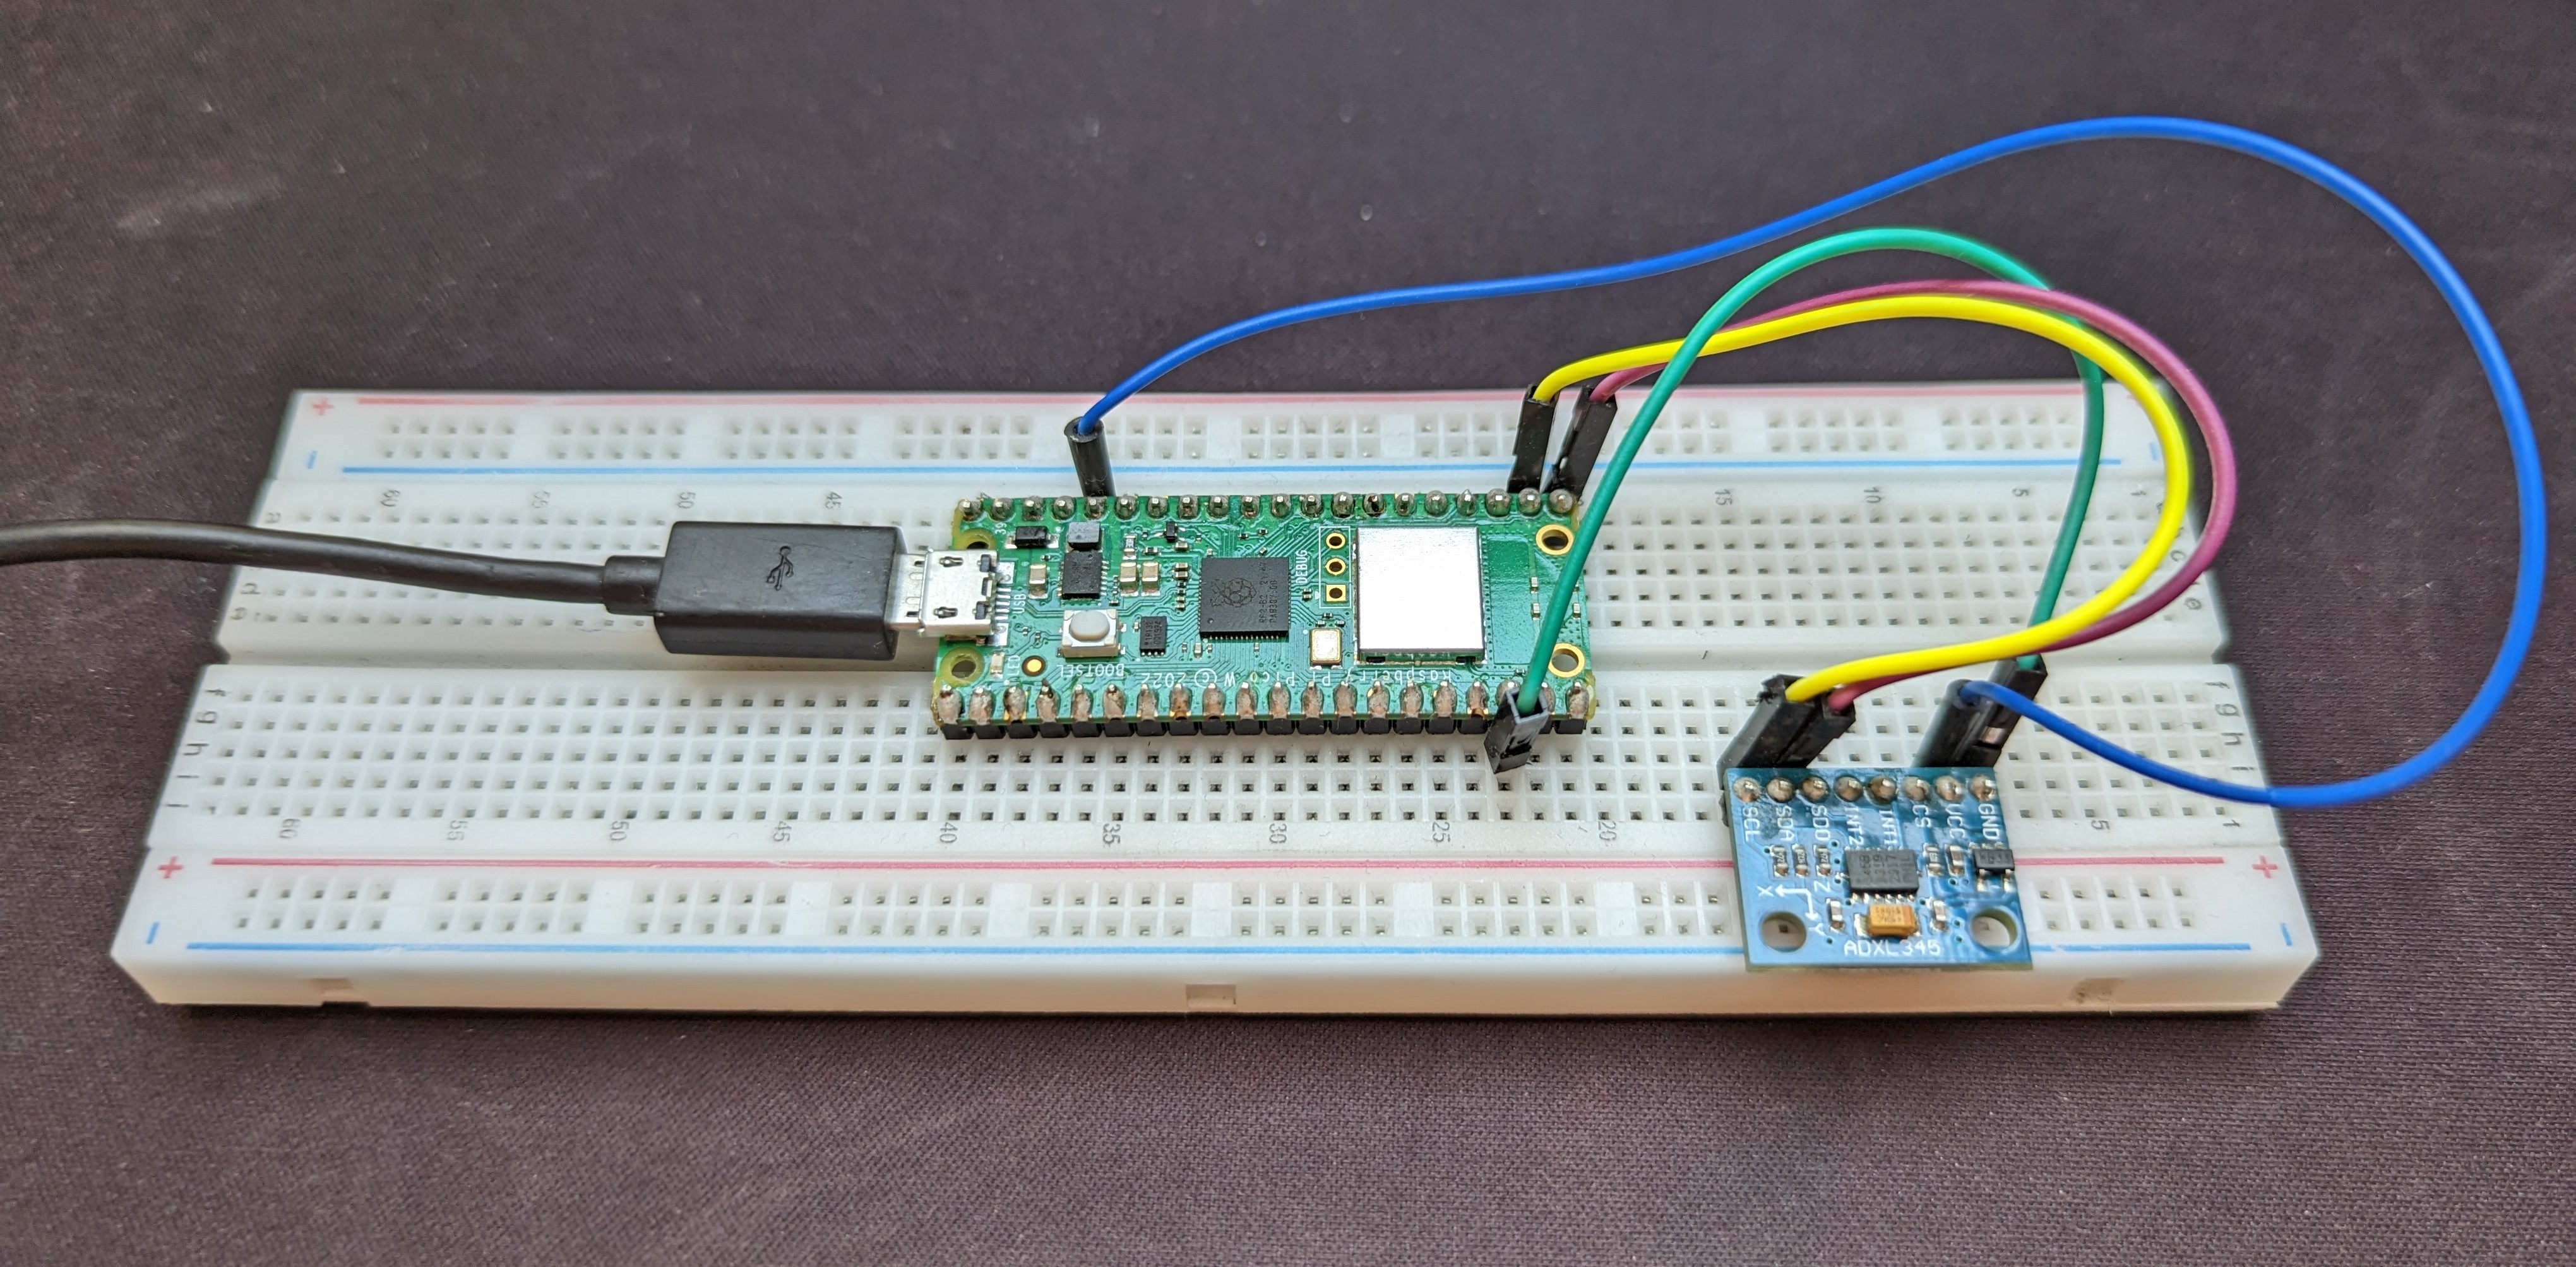
\includegraphics[scale=0.1]{4}
\end{figure}

	\end{appendices}
\end{document}
